% ЕМТ 2024, XII клас — точен LaTeX препис от официалните файлове в Klasirane.com.
% Условия: https://klasirane.com/api/competitions/EMT/All/2024/12%20%D0%BA%D0%BB/probs
% SHA-256 (условия): c15e46d5df8c68c9f3042f7ad948dd40c8a404a090159c2739f7d2016f527940
% Решения: https://klasirane.com/api/competitions/EMT/All/2024/12%20%D0%BA%D0%BB/sol
% SHA-256 (решения): 6ef37deb75f2781441eae92e1e9ba5f979b4952eed9af1ab1bc719ffdbb38e3a
% Точковите оценки, правописът, формулировките и видимите печатни неточности са запазени от източника.
% Файловете са сканирани изображения; всички видими страници са проверени пряко.
% Първата страница на файла с решенията е заглавна и не съдържа условия или решения.

Задача 12.1. Редицата $(a_n)_{n=0}^{\infty}$ е зададена чрез

$$
a_0=c,
$$

$$
a_{n+1}=a_n^2+\frac{a_n}{2}+c\text{ за }n\geq0,
$$

където $c>0$ е реален параметър. Да се намерят всички стойности на $c$, за които редицата $(a_n)$ е сходяща и при тези стойности да се определи нейната граница.

Отговор. $c\in(0,1/16]$.

Решение. Нека първо $c>\frac1{16}$. Тогава имаме

$$a_{n+1}=a_n^2+\frac1{16}+\frac{a_n}{2}+c-\frac1{16}\geq a_n+\left(c-\frac1{16}\right),$$

т.к $x^2+\frac1{16}\geq\frac x2$ за всяко $x\in\mathbb R$. Така получаваме, че $a_n\geq c+(n-1)(c-\frac1{16})$ за $n\in\mathbb N$, т.е редицата е неограничена и следователно не е сходяща.

Обратно, нека $c\leq\frac1{16}$. Ще докажем с индукция по $n$, че за всяко $n\in\mathbb N$ е в сила $a_n\geq a_{n-1}$ и $a_n\leq l$, където $l$ е по-малкият корен на уравнението $f(x)=x^2-\frac x2+c=0$. За $n=0$ е ясно, че $a_1>c=a_0$, а т.к $f(c)=c^2+\frac c2>0$ и $c$ е по-малко от поне един от двата корена на $f$ (това е вярно т.к уравнението има поне един корен по-голям от $1/4$ от формулите на Виет) то следва, че $c<l$.

Ако допуснем, че твърдението е вярно за $n$, то т.к имаме $a_{n+1}-a_n=f(a_n)$, получаваме, че $f(a_n)>0$, понеже $a_n<l$. Също така имаме, че

$$a_{n+1}=a_n^2+\frac{a_n}{2}+c\leq l^2+\frac l2+c=l,$$

където първото неравенство следва, т.к $x\mapsto x^2+\frac x2$ е растяща в $(0,1)$, а последното равенство следва от $f(l)=0$. Така индукцията е завършена откъдето следва, че $a_n$ е растяща и ограничена, следователно сходяща. Ако $t$ е границата ѝ, то $f(t)=0$ и т.к $a_n<l$ за всяко $n\in\mathbb N$, то получаваме, че

$$\lim_{n\to\infty}a_n=l=\frac14-\sqrt{\frac1{16}-c}.$$

Оценяване. (6 точки) 3 т. за $c\leq1/16$, 2 т. за доказване, че ако $c\leq1/16$, то $a_n$ е растяща, 1 т. за довършване.

Задача 12.2. Даден е $\triangle ABC$ и точка $X$ е във вътрешността му. Нека точките $S_A$, $S_B$ и $S_C$ са средите на дъгите $\widehat{BXC}$, $\widehat{AXC}$ и $\widehat{AXB}$ в окръжностите, описани съответно около $\triangle BXC$, $\triangle AXC$ и $\triangle AXB$. Да се докаже, че точките $S_A$, $S_B$, $S_C$ и $X$ лежат на една окръжност.

Решение. Нека $l_A$ е правата през $A$, перпендикулярна на $AX$ и нека $l_B,l_C$ са дефинирани аналогично. Нека $l_B\cap l_C=A_1$, $l_C\cap l_A=B_1$ и $l_A\cap l_B=C_1$. Имаме, че $A_1S_A$ е вътрешната ъглополовяща на $\angle B_1A_1C_1$, т.к $A_1\in(BXC)$. Така получаваме, че правите $A_1S_A,B_1S_B,C_1S_C$ се пресичат в точка $I$, където $I$ е центърът на вписаната окръжност в $\triangle A_1B_1C_1$. Също така имаме, че $A_1X$ е диаметър в $(BXC)$, следователно $\angle IS_AX=90^\circ$, т.е $S_A$ лежи на окръжността с диаметър $IX$. Аналогично получаваме, че точките $S_B$ и $S_C$ лежат на същата окръжност, с което задачата е решена.

Оценяване. (6 точки) 2 т. за построяване на $l_A,l_B,l_C$, 2 т. за доказване, че $A_1S_A,B_1S_B$ и $C_1S_C$ се пресичат в една точка, 2 т. за довършване.

Задача 12.3. Нека $n\geq2$ е естествено число. Ако $m\in\mathbb N$ е такова, че делителите на $m$ могат да се разбият на $n$ непресичащи се множества, така че сумата от числата във всяко множество е една и съща, то да се докаже, че $m\geq2^{n+1}-2$.

Решение. Първи метод. За $n=2$ твърдението се проверява директно. Нататък ще считаме, че $n\geq3$ и $m\geq7$. Да отбележим, че $m$ се среща в някоя от групите, така че $mn\leq\sum_{d\mid m}d$.

Нека $k\in(m/3,m/2)$ е естествено число (такова има поради $m\geq7$). Тогава

$$
\begin{aligned}
mn&\leq\sum_{d\mid m}d=\sum_{d\mid m}\frac md\leq m\left(\sum_{d\leq m,d\mid m}\frac1d\right)\\
&\leq m\left(\sum_{d\leq m/2,d\mid m}\frac1d\right)+1\\
&\leq m\left(\sum_{d\leq m/2}\frac1d\right)-\frac mk+1\\
&<m\left(\sum_{d\leq m/2}\frac1d\right),
\end{aligned}
$$

понеже $m$ няма делители между $\frac m2$ и $m$ и т.к $k$ не дели $m$.

От друга страна имаме, че ако $t\in\mathbb N$ е такова, че $2^t\leq m<2^{t+1}$, то

$$
\sum_{d\leq m/2}\frac1d\leq\sum_{d<2^t}\frac1d
=\sum_{s=0}^{t-1}\sum_{d=2^s}^{2^{s+1}-1}\frac1d
\leq\sum_{s=0}^{t-1}\sum_{d=2^s}^{2^{s+1}-1}\frac1{2^s}=t.
$$

Така получаваме, че $t>n$, откъдето следва, че $m\geq2^{n+1}$.

Коментар. Оценката не е точна, може да се покаже, че $\sum_{d\mid m}d=O(m\log\log m)$. Ето един възможен начин:

Втори метод. (Д.Грозев) Да означим с $s(x)$ сумата от делителите на $x\in\mathbb N$. Имаме $s(m)\geq mn$. Нека $m=p_1^{a_1}p_2^{a_2}\cdots p_k^{a_k}$, където $p_i$ са различни прости числа и $a_i\geq1$. Имаме

$$s(m)\leq m\prod_{i=1}^k\sum_{j=0}^{\infty}\frac1{p_i^j},$$

защото всеки делител на $m$ присъства в дясната страна. И така,

$$s(m)\leq m\prod_{i=1}^k\left(1+\frac1{p_i-1}\right)\leq m\cdot\exp\left(\sum_{i=1}^k\frac1{p_i-1}\right).$$

Тук използвахме неравенството $1+x\leq e^x$. Нататък,

$$\sum_{i=1}^k\frac1{p_i-1}\leq\sum_{i=1}^k\frac1{q_i-1}\leq\sum_{i=1}^k\frac1i<\ln(k+1)\tag{1},$$

където $q_1,q_2,\ldots,q_k$ са първите $k$ прости числа. Това дава $mn\leq s(m)<m(k+1)$ или $k>n-1$, значи $k\geq n$. При $n\geq3$ получаваме

$$m\geq\prod_{i=1}^kq_i\geq2\cdot3\cdot5^{k-2}\geq6\cdot5^{n-2}>5^{n-1}>2^{n+1}.$$

При $n=2$ имаме $k\geq2$ и $m\geq2\cdot3=6$. Вижда се, че $n=2,m=6$ възможно, другите опции са $n=2,m\geq12$ (ако въобще има такива.)

Коментар. Оценката в (1), може да се подобри така

$$\sum_{i=1}^k\frac1{q_1-1}\leq1+\sum_{i=1}^{k-1}\frac1{q_k}\leq1+1+\ln\ln k.$$

Така получаваме, $mn\leq s(m)\leq me^2\ln k$ и значи $\ln k\geq n/e^2$, $k\geq e^{n/9}$ и

$$m\geq\prod_{i=1}^kq_i\geq2^k\geq2^{e^{n/9}}.$$

Също може да се докаже, че

$$\sum_{d\mid m}d\leq H_m+\log H_m e^{H_m},$$

където $H_m=\sum_{i=1}^m\frac1i$.

Оценяване. (7 точки) 1 т. за $mn\leq\sum_{d\mid m}d$, 3 т. за подходяща нетривиална оценка за $\sum_{d\mid m}d$, 1 т. за $m$ няма делител в $(m/2,m)$ и $(m/3,m/2)$, 2 т. за довършване. Случаят $n=2$ не носи точки!

Задача 12.4. Нека $L$ е фигурата, съставена от 3 единични квадрата, четвърт кръг с радиус 1 и правоъгълен равнобедрен триъгълник с катет 1, скачени така:

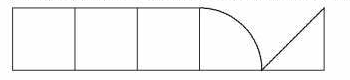
\includegraphics[max width=0.42\textwidth, alt={Официалната фигура L към задача 12.4, съставена от три квадрата, четвърт кръг и правоъгълен равнобедрен триъгълник}, center]{assets/12-4-shape.svg}

Да се докаже, че всеки 18 точки в равнината могат да се покрият с копия на $L$, които не се припокриват в свои вътрешни точки. (Копията на $L$ могат да бъдат ротирани и обръщани.)

Решение. Да разгледаме следната фигура $M$, получена чрез залепяне на 2 копия на $L$.

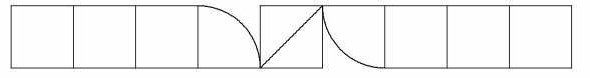
\includegraphics[max width=0.72\textwidth, alt={Официалната фигура M към решение 12.4, получена чрез залепяне на две копия на L}, center]{assets/12-4-double-shape.svg}

Имаме, че $M$ се съдържа в правоъгълник с размери $1\times9$ и заема повече от $17/18$ от лицето му. Нека $S$ е множество от 18 точки в равнината и нека $C$ е случайно покриване на равнината с правоъгълници $1\times9$. По-конкретно фиксираме покриване $A$ на равнината с правоъгълници $1\times9$ и избираме $X\sim U[0,9]$, $Y\sim U[0,1]$, а след това получаваме $C$ като транслираме $A$ с $X$ единици в $x$ направлението и $Y$ единици в $y$ направлението. Всяко такова покриване на равнината дава еднозначно определено покритие на част от равнината с копия на $M$.

Да отбележим, че за всяка точка $s\in S$ имаме

$$\mathbb P(s\text{ е покрита от някое копие на }M)>17/18.$$

Така получаваме, че $\mathbb P(s\text{ не е покрита от копие на }M)<\frac1{18}$. Следователно

$$
\begin{aligned}
\mathbb P(\exists\ s\in S:s\text{ не е покрита от копия на }M)
&\leq\sum_{s\in S}\mathbb P(s\text{ не е покрита от копия на }M)\\
&<|S|/18=1,
\end{aligned}
$$

откъдето следва, че съществува покриване на равнината, за което всяка точка от $S$ е покрита от някое копие на $M$.

Оценяване. (7 точки) 2 т. за разглеждане на $M$, 5 т. за довършване. 3 т. за доказване на по-слабо твърдение като „всеки 8 точки в равнината могат да се покрият с копия на $L$“ чрез вероятностен метод.

Задачите са предложени от: 8.1 и 8.4 – Ивайло Кортезов; 8.2 и 8.3 – Мирослав Маринов; 9.1 и 9.4 – Константин Делчев; 9.2 и 9.3 – Любен Балтаджиев; 10.1 – Станислав Харизанов; 10.2, 10.3 и 10.4 – Божидар Димитров; 11.1 и 11.2 – Емил Колев; 11.3 – Cristi Savescu; 11.4 – Марин Христов; 12.1, 12.2, 12.3 – Кристиан Василев; 12.4 – Teun Verstraaten.
